\chapter{Finding New Sources in POSSUM Data}
\label{ch: sourcefinding}

The following chapter describes my investigation into a possible cause for the lack of rotation measure found within the diffuse emission of the Galactic plane and trialling a potential solution. This investigation was carried out on data produced by the POSSUM collaboration and the field chosen was EMU1505-60. This field was chosen as it crossed a significant amount of Galactic plane compared to the other fields available.

One possible reason for the low RM density in along the Galactic plane is that the areas covered by diffuse emission that spreads across the Galactic plane is interpreted as regions of low signal to noise ratio by the source finder. This results in fewer sources being detected in these regions and thus fewer RM. Another possibility is that the sources within the Galactic plane are depolarised, so their RM is more difficult to detect. This research focuses on addressing the first reason and devising a method to reduce noise and increase the source density.

%pretty sure thats not quite right and that last sentence needs work! also i think this should be in the introduction


% Why it is useful
% How it is done

In order to complete any analysis of sources within radio interferometric data, the positions of these sources must be accurately found. Therefore reliable and accurate source finding methods are key to any sort of radio astronomy. As the capabilities of interferometers has  increased, the number of sources visible in images has also increased and for many years now a manual approach has been unfeasible. Therefore, a variety of different automated software packages have been developed over the last 60 years. The technique most used by these programs is based on the idea of fitting two-dimensional Gaussians to areas that have emission above a given threshold. This method extracts information about both the location and intensity each source. A catalogue of this information is then output as the result for a given image.

\section{Initial Source List}

As part of the ASKAP Observatory pipeline which is run on each POSSUM field prior to data release, a source list for the field was generated using the the source finding software Selavy (\cite{Selavy_Whiting_2012}). This found a total of 10881 components, which can be seen in Figure \ref{fig: validation_selavy}. These point sources are mostly radio galaxies, but there are other extended sources such as a pulsar wind nebula and multiple supernova remnants, most notably the supernova remnant MSH 15-22 (see Figure \ref{fig:sn remnant}) that have been detected as groups of point sources. 


\begin{figure}

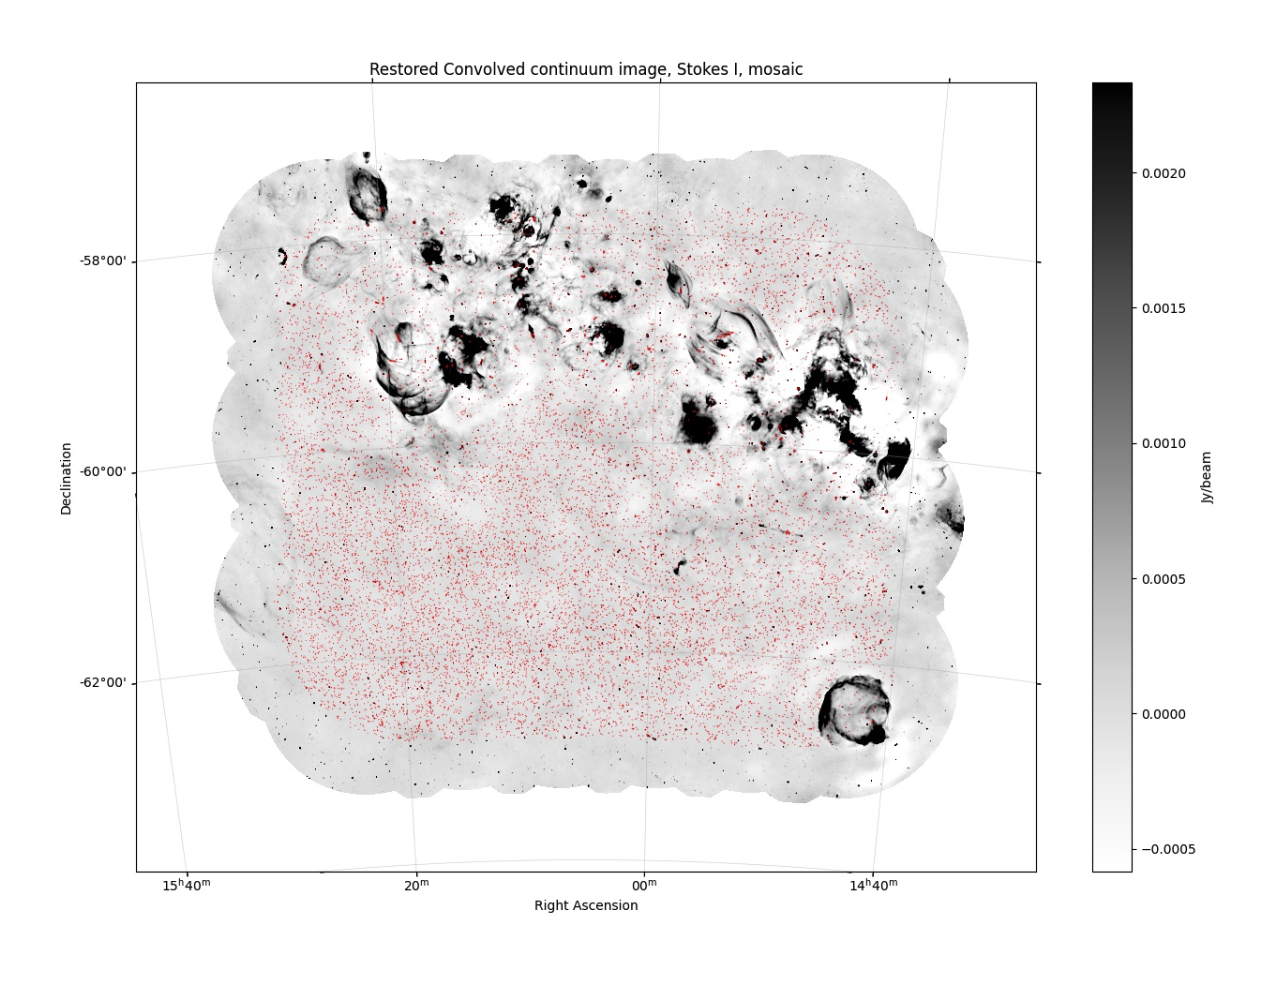
\includegraphics[width=\linewidth]{Thesis_Template/Figures/validation_sourcefinder.png}
\caption{Source catalogue output by Selavy as part of ASKAP Observatory pipeline, produced by \cite{validation}, with each point mapped as a red dot, and the intensity of the field image shown by the grey scale}
\label{fig: validation_selavy}
\end{figure}

\begin{figure}
    \centering
    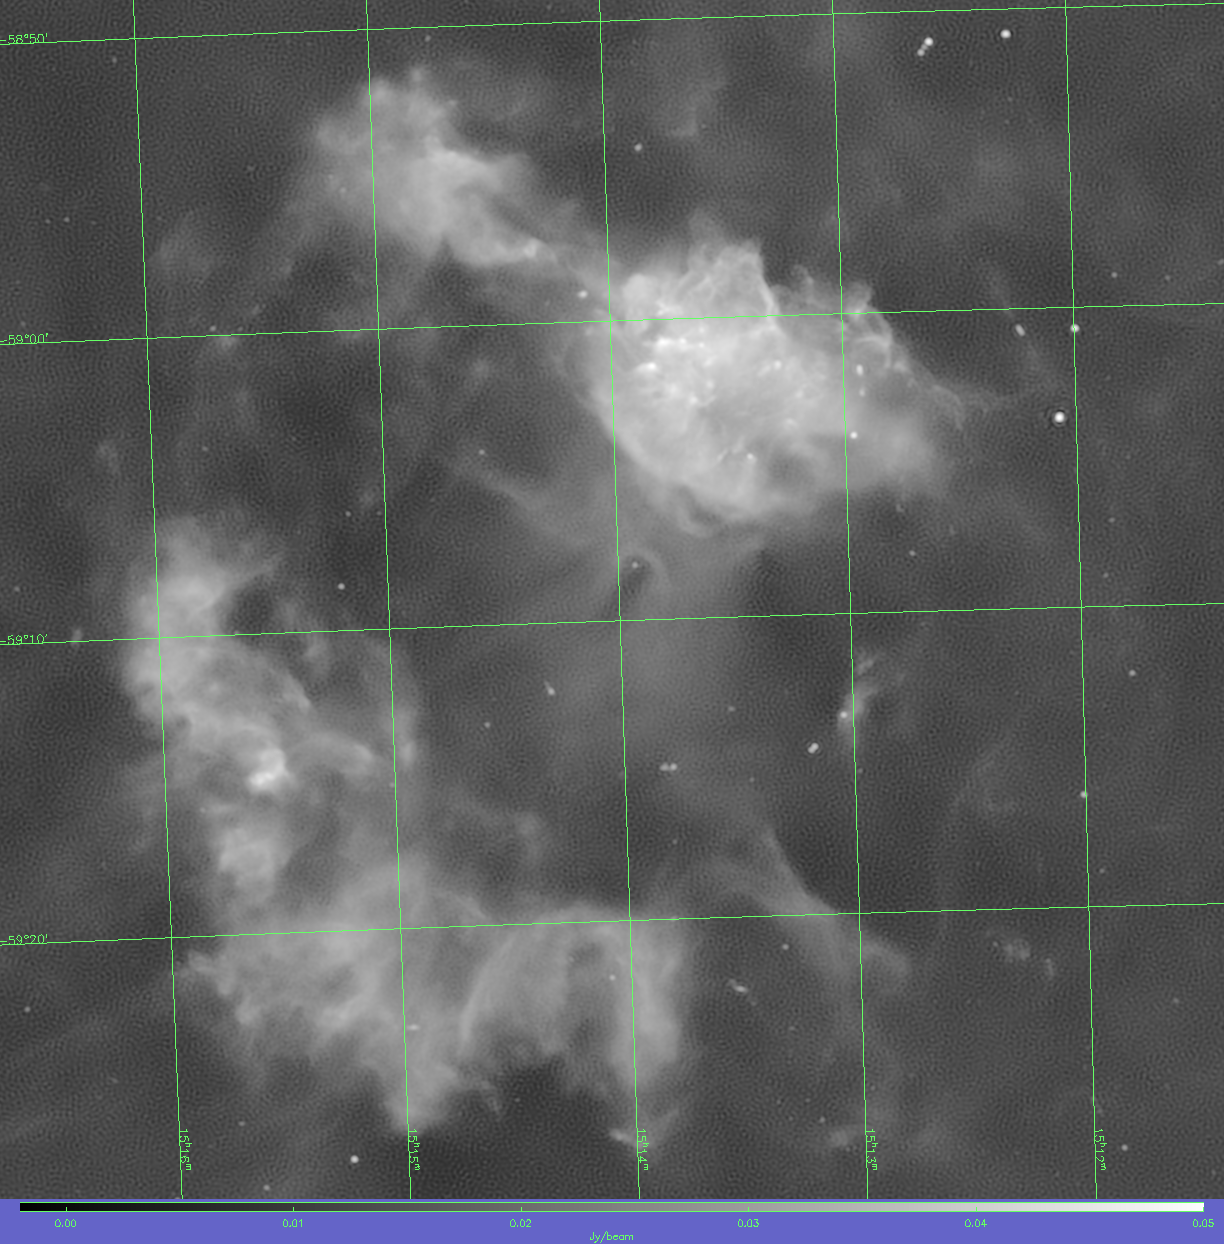
\includegraphics[width=\linewidth]{Thesis_Template/Figures/MSH22-15 hires.png}
    \caption{Zoomed in image of the supernova remnant MSH 15-22 in the hires image using an asinh greyscale which runs from linear near zero and logarithmic for bright emission to highlight all the structure within the nebula}
    \label{fig:sn remnant}
\end{figure}

Selavy is an implementation of the Duchamp source finder (\cite{Duchamp_Whiting_2012}) with additional features designed for ASKAP. Duchamp was initially developed to process three-dimensional spectral line cubes, but could also handle one and two dimensional data sets. 

Much like in Figure \ref{fig: Shannon's RM grids}, it is apparent in Figure \ref{fig: validation_selavy} that there is a distinct lack of sources found along the Galactic plane. There is a stark difference in source density between on and off the Galactic plane, which is demonstrated by Figure \ref{fig:source density in selavy}. The two boxes show the sources within that region with the upper box located on the Galactic plane and the lower box located in an area without diffuse emission. The source density within the diffuse emission is 78 sources per square degree whereas without any diffuse emission the source density is nearly five times greater at 387 sources per square degree. Some of the sources within this area may however be peaks within the nebula of the supernova remnant within this field, which can be seen in greater detail in Figure \ref{fig:sn remnant}.

\begin{figure}
    \centering
    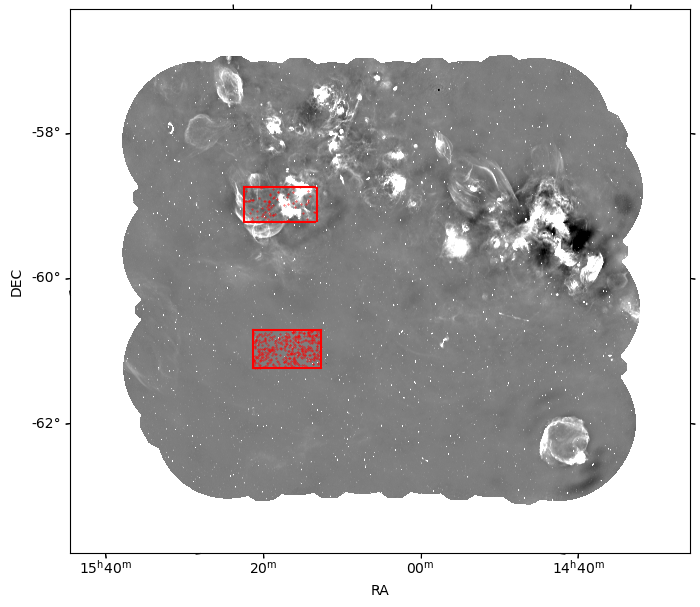
\includegraphics[width=1\linewidth]{Thesis_Template//Figures/selavy_source_density.png}
    \caption{Source Density Comparison of Selavy catalogue between on and off the Galactic Plane}
    \label{fig:source density in selavy}
\end{figure}

The vast majority of the radio sources found by Selavy are extragalactic so we would expect a near-uniform density of sources across all Galactic latitudes, except for minor fluctuations due to the structure of the cosmic web and rare instances of sufficiently compact Galactic sources, such as radio stars, pulsars or peaks in nebulae. Therefore, an explanation is required for this disparity.


\section{Re-Processing} 

In order to reduce the noise, so that more sources can be detected within the diffuse emission, I have reprocessed the image given to the source finder in order to improve the visibility of the sources by removing as much diffuse emission as possible.

When I began this process, I decided to use the higher resolution image produced by EMU. This was the first step in suppressing the noise created in the image by the diffuse emission. When comparing the standard resolution image, Figure \ref{fig: low_res}, with the high resolution image, Figure \ref{fig: high res}, it is clear that the apparent brightness of the diffuse emission is reduced. Another key difference is that the negative 'bowl' artefacts, which are caused by missing short spacings are reduced as the uniform weighting gives higher weight to the short baselines, thus picking up extended structure. One disadvantage however is that the noise is increased and there stippled noise pattern which is not present in the low resolution image. Moreover, after CLEANing to a fixed threshold, extended nebulae retain much flux density within the dirty map and as it has not been deconvolved and is only detected on a few short baselines, large sidelobes remain.

\begin{figure}
    \centering
    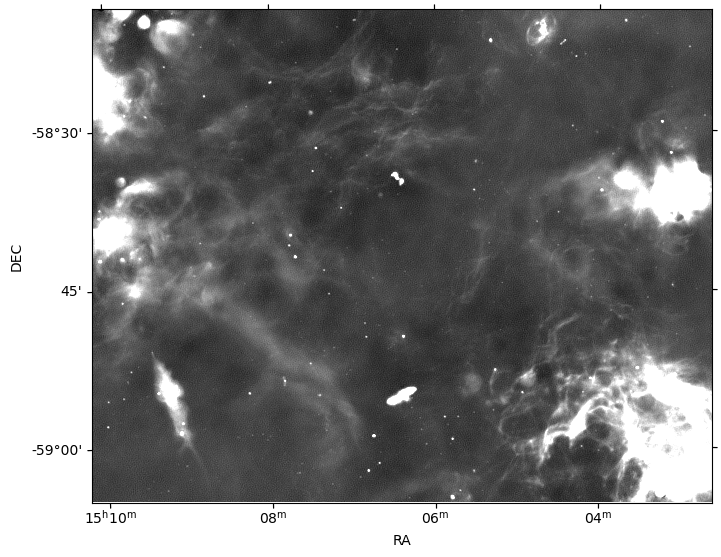
\includegraphics[width=1\linewidth]{Thesis_Template//Figures/high_res_crop.png}
    \caption{Cropped high resolution image of the EMU1505-60 field.}
    \label{fig: high res}
\end{figure}


\begin{figure}

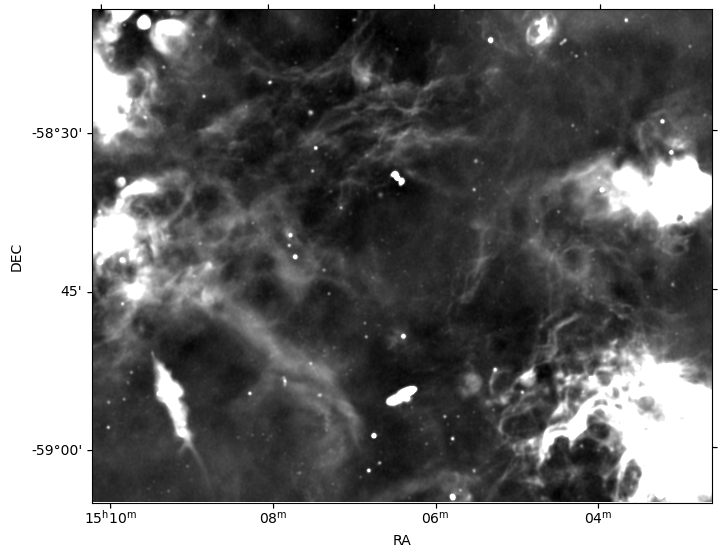
\includegraphics[width=1\linewidth]{Thesis_Template/Figures/lo.png}
\caption{Low resolution, or standard, image of field EMU1505-60.}
\label{fig: low_res}
\end{figure}


The region around the edge of each individual POSSUM field has high noise due to the primary beam correction. To remove this, I created a subsection of the image, and subsequently each Stokes parameter cube, using AIPS. The size of this section was chosen to have dimensions of $8192{\rm \, x\,}8192$ pixels because a power-of-two size will speed up the Fourier transform performed for RM synthesis.


\subsection{Masking}

In order to suppress the diffuse galactic emission I used the AIPS program NINER to apply a peak finding filter. This served to highlight the point sources and reduced the apparent brightness of the large scale galactic structure. NINER works by convolving the image with a 3 x 3 matrix. 

The matrix used was that shown below.


\begin{equation}
    \begin{bmatrix}

    -1 & -1 & -1\\
    -1 & 8 & -1\\
    -1&-1&-1
    
    \end{bmatrix}
    \label{eq: msk2}
\end{equation}

This process successfully suppressed the diffuse emission, leaving behind a field dominated by point sources (Figure \ref{fig: niner}). This does however greatly increase the noise, as this image has a background rms of $200 \,\mu{\rm Jy}$, which is almost six times that of the standard image. This affects the flux measured for each source. The next step was to use a source finding algorithm to locate these sources.

% ppp add figure of niner result

\begin{figure}
    \centering
    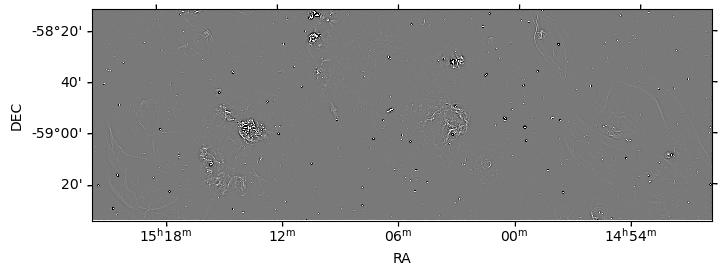
\includegraphics[width=1\linewidth]{Thesis_Template/Figures/niner.png}
    \caption{A zoom in of the NINER output image showing the point sources highlighted by this convolution process}
    \label{fig: niner}
\end{figure}



\section{Source Finding Algorithms}

There are many source finding algorithms available, each with their own strengths and weaknesses, so a decision had to be made as to which one to use. The source finder used in the ASKAP Observatory pipeline is Selavy. This source finding algorithm works by grouping pixels in an image that are three times the root-mean-square (rms) of the image, and then fitting a Gaussian to peaks within the islands, with only peaks with an intensity of above five times the rms being counted as sources. The rms is found by calculating the median absolute deviation from the median (MADFM) and the same value is applied across the entire image. MADFM was chosen as a proxy for standard deviation due to its robustness against bright pixels which would otherwise contribute to the background noise calculation (\cite{Duchamp_Whiting_2012}). 

To help find which would be the most suitable tool, I referred to the results of The ASKAP/EMU Source Finding Data Challenge (\cite{data_challenge}). This was an investigation carried out by POSSUM's sister survey EMU with the aim of assessing the various merits and downfalls of many source finding algorithms currently available. The challenge involved creating three artificial source lists and images with source brightness and quantity of extended sources which many source finders, including Selavy, were then run on. The results from each source finder were then compared by quantifying their accuracy and identifying their limitations. 

The Python Blob Detector and Source Finder (PyBDSF)\footnote{PyBDSF can be accessed at https://github.com/lofar-astron/PyBDSF/tree/master} showed high completeness whilst also maintaining high reliability in the fainter, psuedo-realistic catalogue they had generated. Selavy, however, showed a very low reliability in this challenge. Furthermore, Selavy would be difficult to implement as it is currently only available as part of the data processing pipeline, whereas PyBDSF could be installed separately. Therefore, I made the decision to use PyBDSF instead.

PyBDSF (\cite{PyBDSF}) works by first calculating the background rms and mean images, which is done by using a box of a sensible size, which was chosen to be 819x819 pixels, and calculating the mean and standard deviation within the box at multiple places across the image with a step size of 273 pixels. Outliers are then excluded and the process is repeated iteratively until a constant value is reached. A threshold between background and source is set and then islands made of adjacent point sources are found. The threshold can be chosen to be either hard thresholding or using the False Detection rate method, or if it is not set, the program chooses the most appropriate based on the ratio of expected false pixels to true pixels. The hard thresholding was chosen by the program, which uses a 5-sigma for the pixel threshold and 3-sigma for the island boundaries. These islands are then simultaneously fit with multiple Gaussians with the number of Gaussians fit is determined by the number of distinct peaks, with a peak being defined by having a negative gradient in all eight directions. Then, those Gaussians are grouped into discrete sources. Groups within these islands are considered a discrete source if they are obviously distinct on the image. This distinction is calculated as if the difference between the peak of the lower Gaussian and the minimum value directly between the centre of each Gaussian is less than the product of the island threshold and the island rms and the distance between peak centres is less than half the sum of their full width half maximum value along the line joining them then they are categorised as the same source. The location and size of that source is then found by moment analysis %do I need to explain moment analysis?
and the flux found by the sum of the Gaussians within the source.

As the final step towards producing the improved source list, I ran PyBDSF on the processed image. This then produced a catalogue of sources, with location and intensity information. The sources found can be seen in Figure \ref{fig:pybdsf sourcelist}. This is another benefit of PyBDSF as it produces a list of sources and Gaussian components, for which I used the list of sources for further analysis, whereas Selavy only produces a list of Gaussian components which then have to be later grouped into sources by the user.

\begin{figure}
    \centering
    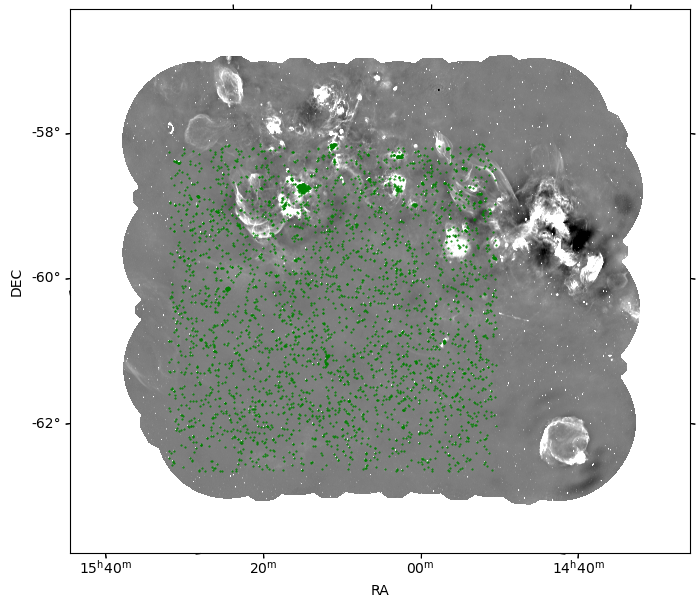
\includegraphics[width=\linewidth]{Thesis_Template/Figures/PyBDSF_sources.png}
    \caption{All sources found by the PyBDSF source finding algorithm when run on the reprocessed image}
    \label{fig:pybdsf sourcelist}
\end{figure}


\section{Comparison of Source Catalogues}

In order to find if an improvement had been made by using the method outlined here, I conducted some comparisons between the original catalogue produced by Selavy during the observatory pipeline processing and the PyBDSF catalogue.

The first comparison I made was to see whether there has been a net increase in sources within the field processed with this method. I found that the source list created by PyBDSF after the reprocessing found fewer sources than the same subsection in Selavy.  However, this is to be expected, as the high resolution image has higher noise than the low resolution used for initial source finding, and moreover the implementation of NINER further increased the noise level throughout the image. The increase in noise from this process has affected the flux found by the source finder. By picking three point sources and comparing the flux measured by for that source by both Selavy and PyBDSF I have found that there is on average a 32$\%$ increase in flux from the Selavy to the PyBDSF catalogue.

To make a useful comparison I have focused my comparative efforts on the region shown in Figure \ref{fig: comparison_blank}. This region was chosen to cover as much of the diffuse emission as possible without including excess regions of clear sky so that the difference can be clearly measured.

\begin{figure}

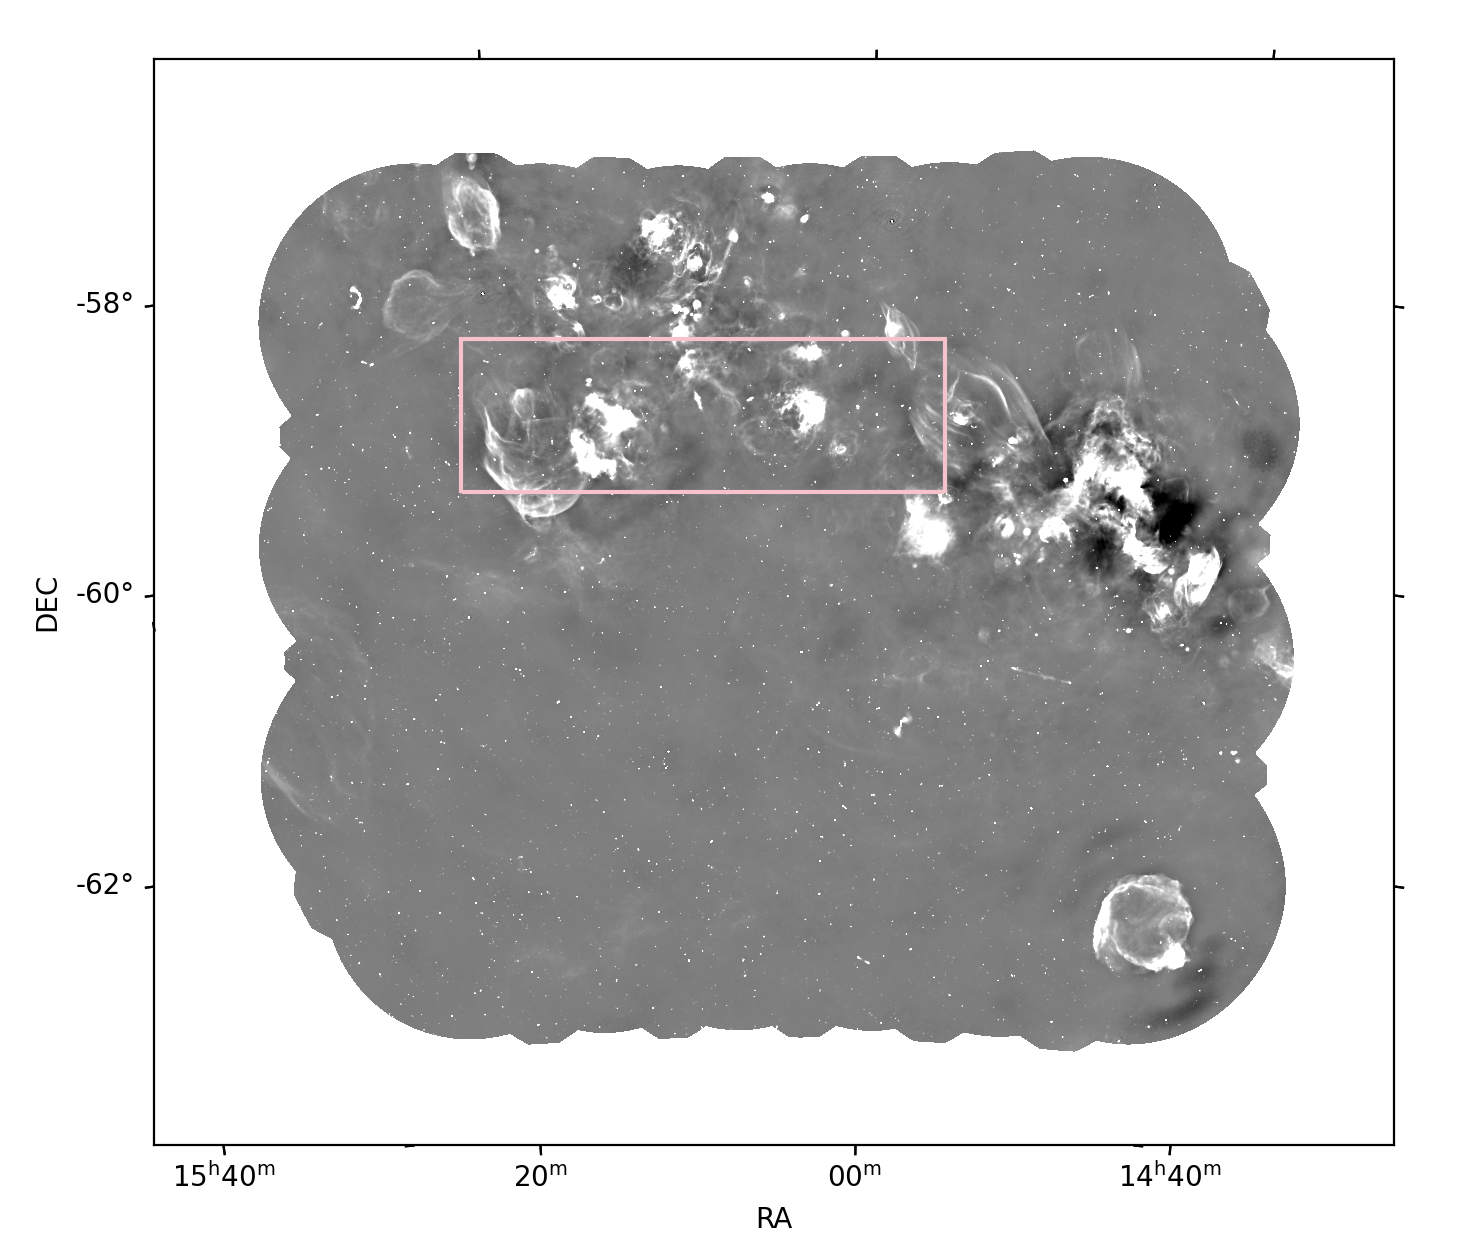
\includegraphics[width=0.9\linewidth]{Thesis_Template/Figures/comparison region.png}
\caption{\small Region within field EMU1505-60 chosen for comparison between the source list produced for this project and the source list produced as part of the observatory pipeline for the field.}
\label{fig: comparison_blank}
\end{figure}

Within this comparison region, the Selavy catalogue contains 650 sources, whereas the PyBDSF catalogue contains 854 sources. This shows a significant increase in sources detected within the Galactic plane.

I then assessed whether the sources were aligned between the two catalogues. To do this, I converted the position from Right Ascension and Declination into Cartesian coordinates for each source in the comparison region. I then calculated the separation between each pair of sources between the catalogues. I considered each pair of sources that are within 5 arcseconds of each other to be the same source. By pairing the sources in this way I found that there were sources from both catalogues which didn't appear to have a match by this method. There were 509 sources that were found by PyBDSF and not Selavy, which can be seen in Figure \ref{fig: pybdsf not match}, and 345 sources that were found by Selavy but not PyBDSF, which can be seen in Figure \ref{fig: selavy not match}. The sources that were not found by PyBDSF in this region are mainly within areas of the comparison region that do not have much diffuse emission, and the opposite is true for the sources not found in the Selavy catalogue. This suggests that the method culminating in the PyBDSF source catalogue has successfully increased source finding within the diffuse emission of the Galactic plane.

\begin{figure}
    \centering
    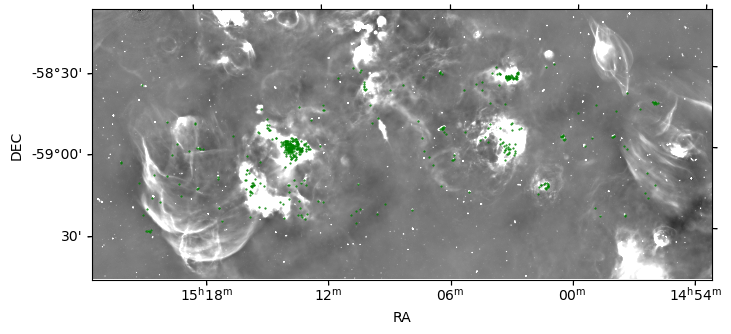
\includegraphics[width=\linewidth]{Thesis_Template/Figures/Py match.png}
    \caption{Sources in the PyBDSF catalogue that were not within 5 arcseconds of a source in the Selavy catalogue}
    \label{fig: pybdsf not match}
\end{figure}

\begin{figure}
    \centering
    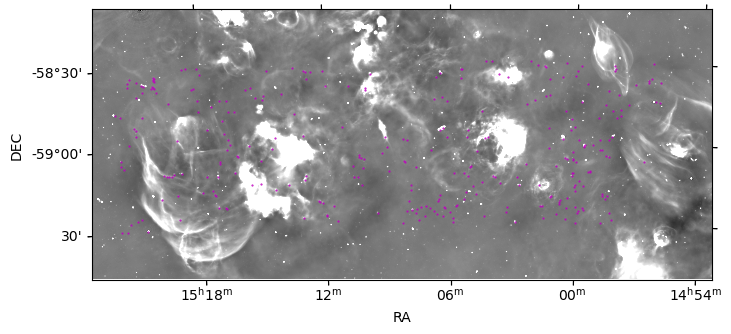
\includegraphics[width=\linewidth]{Thesis_Template/Figures/sel match.png}
    \caption{Sources in the Selavy catalogue that were not within 5 arcseconds of a source in the PyBDSF catalogue}
    \label{fig: selavy not match}
\end{figure}

I also calculated the source density both on and off the Galactic plane in the same regions used for this calculation on the Selavy catalogue. This showed great improvement in source density for the region in within the diffuse emission, with a density of 249 sources per square degree. This is over a 200$\%$ increase from the Selavy catalogue. There was, however, a decrease in source density off the Galactic plane, with a source density of 101 sources per square degree.

It is also worth noting that there is an over-density of PyBDSF sources in the bright region of the supernova remnant MSH15-22 and in the nebula at RA 15:03 and Dec -58:50. The source finder has mistaken bright emission peaks within the structure of the nebula for extragalactic sources. How the sources have been assigned to this nebula's structure can be seen in finer detail in Figure \ref{fig: snr sources}. Cases where sources are just peaks in brightness within the diffuse emission have been identified and removed from the catalogue via manual inspection.

\begin{figure}
    \centering
    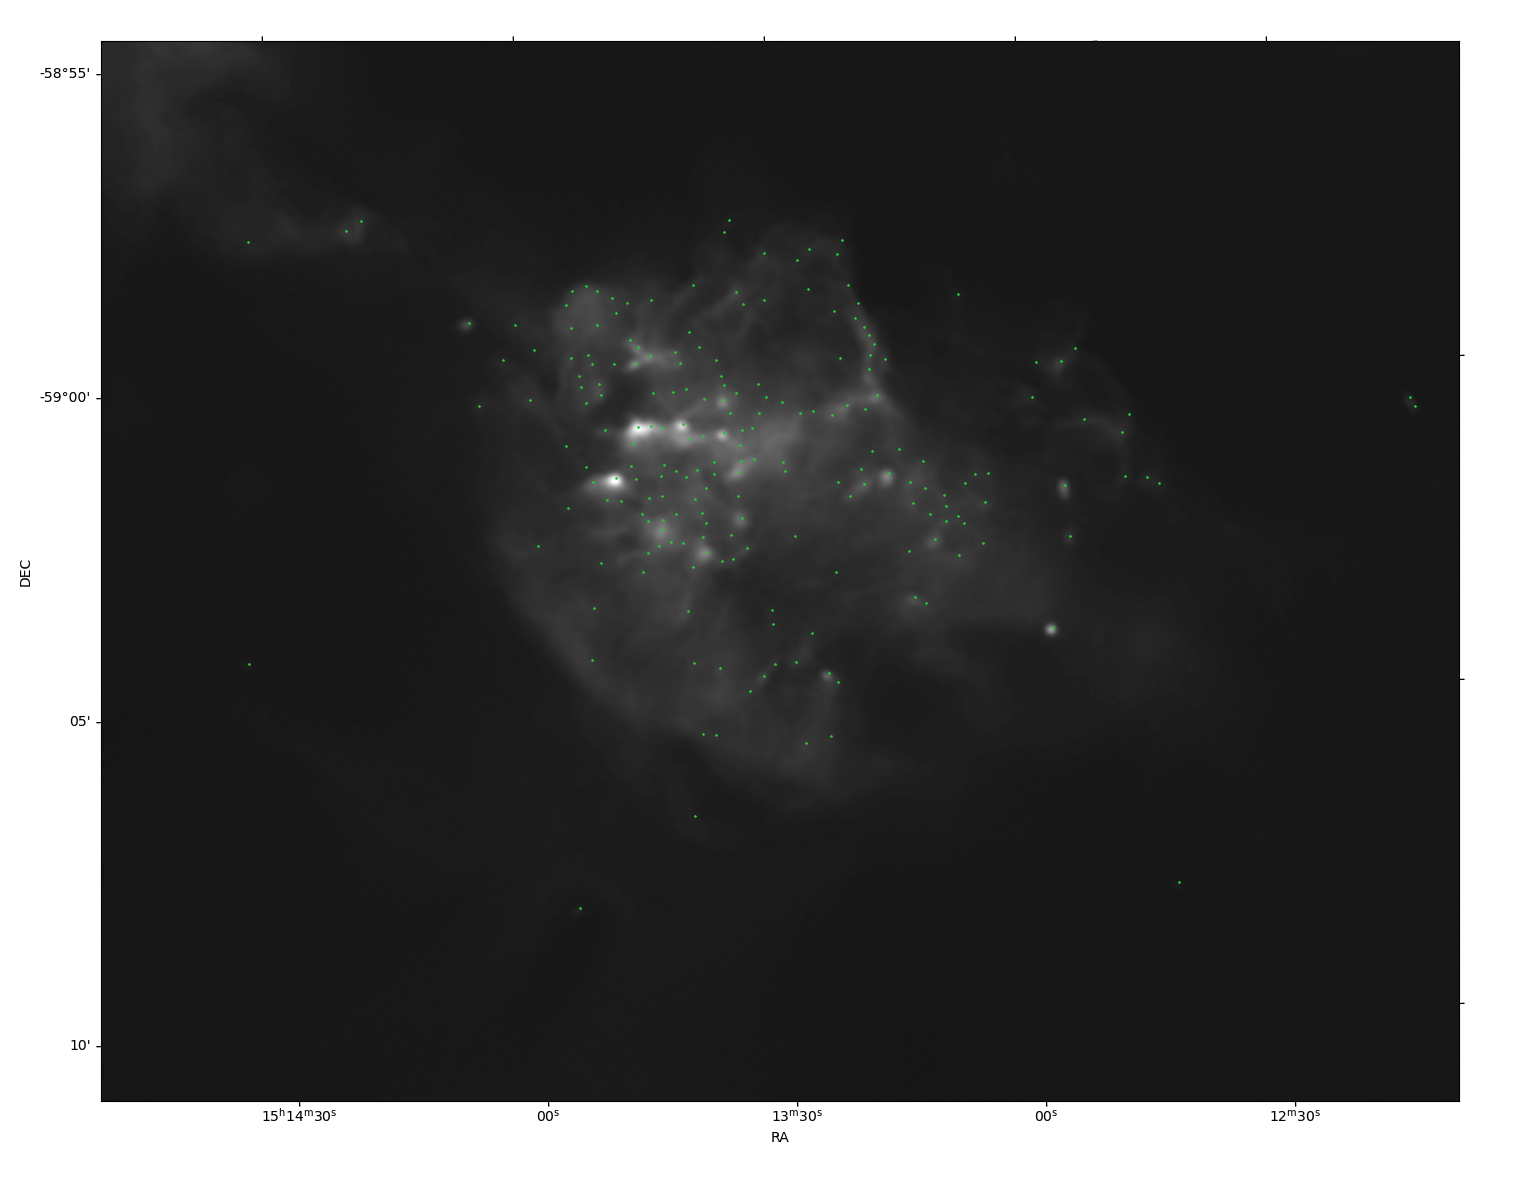
\includegraphics[width=\linewidth]{Thesis_Template/Figures/MSH15-22 sources.png}
    \caption{The supernova remnant MSH 15-22 with the 'sources' identified by PyBDSF}
    \label{fig: snr sources}
\end{figure}

\begin{figure}
    \centering
    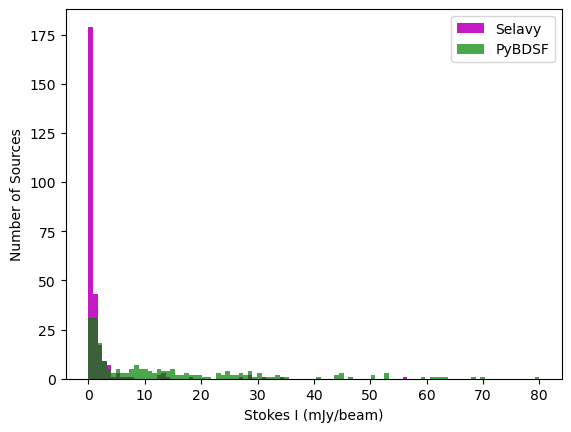
\includegraphics[width=\linewidth]{Thesis_Template/Figures/unmatched histogram.png}
    \caption{Histogram of flux densities for both source finding algorithms, with nebulae brightness peaks removed}
    \label{fig: unmatched histogram}
\end{figure}

Another point of interest, demonstrated in Figure \ref{fig: unmatched histogram}, is that the Selavy catalogue includes significantly more fainter sources, whereas the PyBDSF catalogue has found fewer faint sources but more sources. This histogram excludes the peaks in the brightness of the diffuse emission of the nebulae.

These results demonstrate that the diffuse emission is being interpreted as noise by the source finding algorithm, as this method of convolving the image to smooth the image over the 3 x 3 matrix and highlight point sources has been successful in producing more sources within the Galactic plane. However, this method has been found to decrease source detection within areas without diffuse emission. This is because the the gradient mask highlights sources with a large gradient, which highlights bright sources, but suppresses fainter sources which makes them less visible than they would normally be visible in areas with low noise or no diffuse emission. This means that this method alone is not the optimal method for source finding over all fields and a combination between the initial source finding and this method should be employed.

These additional sources detected within the Galactic plane can then be used to conduct RM synthesis and thus find more RM within the Galactic plane, which will allow insight into the magnetic field of this rapidly varying region of the Milky Way. The next chapter details my implementation of the POSSUM polarimetry analysis pipeline to perform RM synthesis and the results it yielded.